\documentclass{article}

\usepackage[margin=1in]{geometry}
\usepackage{amsmath,amsthm,amssymb}
\usepackage{bbm,enumerate,mathtools}
\usepackage{tikz}

\newenvironment{question}{\begin{trivlist}\item[\textbf{Question.}]}{\end{trivlist}}
\newenvironment{note}{\begin{trivlist}\item[\textbf{Note.}]}{\end{trivlist}}
\newenvironment{related}{\begin{trivlist}\item[\textbf{Related.}]\end{trivlist}\begin{enumerate}}{\end{enumerate}}
\begin{document}

\title{Problem 3.}
\date{}
\author{}
\maketitle

  Let $G$ be some $n \times m$ grid as in Figure 1, where each cell has two
  opposite diagonals connected (uniformly at random).
  A cell is chosen (also uniformly at random), and the segment given by the path of
  diagonals that goes through the selected cell is is inspected.
\begin{figure}[!h]
  \centering
  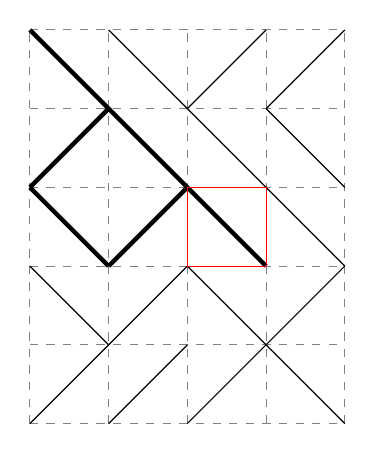
\begin{tikzpicture}
    \draw[thin,gray,dashed] (0,0) grid (4,5);

    \draw[ultra thick] (0,5) -- (1,4);
    \draw[ultra thick] (0,3) -- (1,4); \draw[ultra thick] (1,4) -- (2,3);
    \draw[ultra thick] (0,3) -- (1,2); \draw[ultra thick] (1,2) -- (2,3); \draw[ultra thick] (2,3) -- (3,2);

    \draw (1,5) -- (2,4); \draw (2,4) -- (3,5); \draw (3,4) -- (4,5);
                                                \draw (2,4) -- (3,3); \draw (3,4) -- (4,3);
                                                                      \draw (3,3) -- (4,2);
    \draw (0,2) -- (1,1); \draw (1,1) -- (2,2); \draw (2,2) -- (3,1); \draw (3,1) -- (4,2);
    \draw (0,0) -- (1,1); \draw (1,0) -- (2,1); \draw (2,0) -- (3,1); \draw (3,1) -- (4,0);

    \draw[red] (2,2) -- (2,3);
    \draw[red] (2,3) -- (3,3);
    \draw[red] (3,2) -- (3,3);
    \draw[red] (2,2) -- (3,2);
  \end{tikzpicture}
  \caption{
    An example of a $4 \times 5$ grid, where a segment of size $6$ has been selected.
  }
\end{figure}

\begin{question}
  What is the expected length of the selected segment?
\end{question}

\begin{related}
  \item What is the expected number of segments in an $n \times m$ grid?
  \item How long is the longest segment expected to be?
  \item How does this change if the grid is toroidal, on a cylinder,
    on a M\"obius strip, etc?
\end{related}

\end{document}
